\documentclass{meetings}


\usepackage{makecell}
\usepackage{xcolor}
\usepackage{multirow}
\usepackage{booktabs}
\usepackage{graphicx}
\usepackage{subcaption}
\usepackage{multicol}
\usepackage{tikz}
\usetikzlibrary{positioning}

\setlength{\parskip}{0pt}
\raggedcolumns

\author{S. König, L. Matzner, F. Rollbühler and J. Schmid}
\date{Tuesday, 20\textsuperscript{th} October 2020}


\begin{document}

\section{Introduction}
Graphs are growing fast and are becoming increasingly popular. Many problems can be modeled and solved using graphs.



We compare some state-of-the-art non-uniform memory access (NUMA) aware systems and Giraph in terms of performance, both on real world and synthetic graphs.
Therefore, we evaluate the three algorithms Single-Source Shortest-Paths (SSSP), Breadth-First Search (BFS) and PageRank (PR).
We compare not only the time the frameworks indicate, they need to compute, but also the time they actually run and consume resources, as well as the resulting overhead time.

\clearpage
\section{Overview}


\clearpage
\section{Preliminaries}
\begin{multicols}{2}
A \emph{weighted, directed graph} is the pair $G=(V,E,w)$ where the \emph{vertex set} is $V\subseteq\mathbb N$ and the $E$ is the \emph{edge set} with
	\begin{equation*}
	  E\subseteq\{(x,y)\,|\, x,y\in V, x\neq y\}
	\end{equation*}
	and $w:E\rightarrow \mathbb R$ is a mapping of edge to a weight.
	
	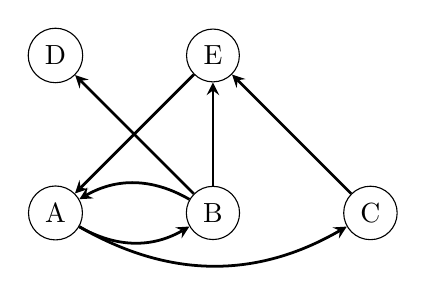
\begin{tikzpicture}
		\node[circle, draw] (a) at (0,0) {A};
		\node[circle, draw] (b) at (2,0) {B};
		\node[circle, draw] (c) at (4,0) {C};
		\node[circle, draw] (d) at (0,2) {D};
		\node[circle, draw] (e) at (2,2) {E};

		\draw[-stealth, bend right, line width=1pt] (a) edge (b);
		\draw[-stealth, bend right, line width=1pt] (a) edge (c);

		\draw[-stealth, bend right, line width=1pt] (b) edge (a);
		\draw[-stealth, line width=1pt] (b) -- (d);
		\draw[-stealth, line width=1pt] (b) -- (e);

		\draw[-stealth, line width=1pt] (c) -- (e);

		\draw[-stealth, line width=1pt] (e) -- (a);
	\end{tikzpicture}


	\columnbreak

	
	Algorithms:
\begin{itemize}
	\item Single-Source Shortest-Paths (SSSP) is the problem of finding the shortest path from a starting vertex to every other vertex in the input graph.

	\item Breadth-first search (BFS) is a search problem on a graph.


	\item PageRank (PR) is a link analysis algorithm that weighs the vertices of a graph, measuring the vertices relative importance within the graph

\end{itemize}
\end{multicols}


\clearpage
\section{Push \& Pull}

\clearpage
\section{Hugepages}


SSSP, BFS, PR, Push/Pull, Hugepages

\clearpage
\section{Frameworks}

\clearpage
\section{Evaluation}
\begin{multicols}{2}
\noindent 5 Machines, with
\begin{itemize}
	\item 96 cores, of which 48 virtual
	\item 256 GB of RAM each, one machine only 128 GB
	\item Ubuntu 18.04.2 LTS
\end{itemize}
\noindent Measurements:
\begin{itemize}
	\item \textbf{execution time}: time from start to finish of the console command
	\item \textbf{calculation time}: time the framework actually executed the algorithm
	\item \textbf{overhead}: time difference between execution time and calculation time \newline (time to read the input graph, initialization, etc.)
\end{itemize}

\renewcommand{\arraystretch}{1.2}%
{%
\noindent
\centering
	\begin{tabular}{crr}
		\hline
		\bf{Graph}&\# Vertices (M)&\# Edges (M)\\\hline
		flickr&    		0.1&  2\\
		orkut&          3&    117\\
		wikipedia&      12&   378\\
		twitter&     	52&   1963\\
		rMat27&         63&   2147\\
		friendster&     68&   2586\\
		rMat28&         121&  4294\\
		\hline
	\end{tabular}
}%

each test case (graph, framework, algorithm) was run 10 times
\end{multicols}



\clearpage
\begin{multicols}{2}
\section{Production Case}
\begin{itemize}
	\item running system, that performs multiple calculations on a single graph
	\item without the need of reloading graph data with every calculation
	\item short calculation times should be preferred because the overhead time is only spent once on startup and amortizes quickly
\end{itemize}

\columnbreak
\section{Research Case}
\begin{itemize}
	\item individual calculations on a graph, i.e. for each calculation, the graph has to be loaded
	\item the algorithm can change frequently
	\item requiring the framework to be relatively fast on different algorithms
	\item overall small execution times and small overhead are preferred
\end{itemize}
\end{multicols}

Messfehlern bei Galois Calc was sagen

\clearpage
\section{Production Case Single Node}

\begin{figure}[h]
	\begin{subfigure}{0.32\textwidth}
		\includegraphics[width=\linewidth]{../../plots/singleNodeSSSP_calcTime.png}
		\caption{SSSP}
	\end{subfigure}
	\begin{subfigure}{0.32\textwidth}
		\includegraphics[width=\linewidth]{../../plots/singleNodeBFS_calcTime.png}
		\caption{BFS}
	\end{subfigure}
	\begin{subfigure}{0.32\textwidth}
		\includegraphics[width=\linewidth]{../../plots/singleNodePR_calcTime.png}
		\caption{PR}
	\end{subfigure}
\end{figure}
\begin{itemize}
	\item Giraph is either very slow or requires too much RAM (>256 GB)
	\item On SSSP, Polymer is fastest, followed by Gemini on second place
	\item On BFS, Gemini and Ligra are comparable and fastest on the larger graphs
	\item On PR, Galois is fastest. But we exclude Galois Push because of possible measuring errors.
	\item Message-based approach can compete with shared-memory
\end{itemize}

\clearpage
\section{Production Case Distributed}

\begin{figure}[h]
	\begin{subfigure}{0.32\textwidth}
		\includegraphics[width=\linewidth]{../../plots/distributedSSSP_calcTime.png}
		\caption{SSSP}
	\end{subfigure}
	\begin{subfigure}{0.32\textwidth}
		\includegraphics[width=\linewidth]{../../plots/distributedBFS_calcTime.png}
		\caption{BFS}
	\end{subfigure}
	\begin{subfigure}{0.32\textwidth}
		\includegraphics[width=\linewidth]{../../plots/distributedPR_calcTime.png}
		\caption{PR}
	\end{subfigure}
\end{figure}
\begin{itemize}
	\item Giraph is fastest on SSSP and BFS on the real world graphs
	\item Giraph has problems with synthetic graphs
	\item Gemini is fastest on PR, with Giraph on second place
\end{itemize}











\section{Research Case Single Node}

\begin{figure}[h]
	\begin{subfigure}{0.32\textwidth}
		\includegraphics[width=\linewidth]{../../plots/singleNodeSSSP_execTime.png}
		\caption{SSSP}
		\label{fig:singleNodeSSSP_exec}
	\end{subfigure}
	\begin{subfigure}{0.32\textwidth}
		\includegraphics[width=\linewidth]{../../plots/singleNodeBFS_execTime.png}
		\caption{BFS}
		\label{fig:singleNodeSSSP_exec}
	\end{subfigure}
	\begin{subfigure}{0.32\textwidth}
		\includegraphics[width=\linewidth]{../../plots/singleNodePR_execTime.png}
		\caption{PR}
		\label{fig:singleNodeSSSP_exec}
	\end{subfigure}
\end{figure}
\begin{itemize}
	\item Giraph is either slowest or requires too much RAM (>256 GB)
	\item Galois is fastest in almost all cases, second fastest is Ligra
	\item Gemini and Polymer are comparably slow
\end{itemize}

\clearpage
\section{Research Case Distributed}

\begin{figure}[h]
	\begin{subfigure}{0.32\textwidth}
		\includegraphics[width=\linewidth]{../../plots/distributedSSSP_execTime.png}
		\caption{SSSP}
		\label{fig:distributedSSSP_exec}
	\end{subfigure}
	\begin{subfigure}{0.32\textwidth}
		\includegraphics[width=\linewidth]{../../plots/distributedBFS_execTime.png}
		\caption{BFS}
		\label{fig:distributedSSSP_exec}
	\end{subfigure}
	\begin{subfigure}{0.32\textwidth}
		\includegraphics[width=\linewidth]{../../plots/distributedPR_execTime.png}
		\caption{PR}
		\label{fig:distributedSSSP_exec}
	\end{subfigure}
\end{figure}
\begin{itemize}
	\item Galois Push is faster than Pull in all cases
	\item Either Galois implementation is faster than any other frameworks on SSSP or BFS
	\item Gemini is fastest on PR and comparable to Giraph on SSSP and BFS
\end{itemize}



\section{Conclusion and Outlook}
Für jeden Fall ist das beste Framework sehr spezifisch.
Blabla.

Outlook:
Immer wieder solche Tests machen, viele der Frameworks ändern sich immer wieder weiter und so, nicht wahr.
\end{document}
